% Options for packages loaded elsewhere
\PassOptionsToPackage{unicode}{hyperref}
\PassOptionsToPackage{hyphens}{url}
%
\documentclass[
]{article}
\usepackage{amsmath,amssymb}
\usepackage{lmodern}
\usepackage{iftex}
\ifPDFTeX
  \usepackage[T1]{fontenc}
  \usepackage[utf8]{inputenc}
  \usepackage{textcomp} % provide euro and other symbols
\else % if luatex or xetex
  \usepackage{unicode-math}
  \defaultfontfeatures{Scale=MatchLowercase}
  \defaultfontfeatures[\rmfamily]{Ligatures=TeX,Scale=1}
\fi
% Use upquote if available, for straight quotes in verbatim environments
\IfFileExists{upquote.sty}{\usepackage{upquote}}{}
\IfFileExists{microtype.sty}{% use microtype if available
  \usepackage[]{microtype}
  \UseMicrotypeSet[protrusion]{basicmath} % disable protrusion for tt fonts
}{}
\makeatletter
\@ifundefined{KOMAClassName}{% if non-KOMA class
  \IfFileExists{parskip.sty}{%
    \usepackage{parskip}
  }{% else
    \setlength{\parindent}{0pt}
    \setlength{\parskip}{6pt plus 2pt minus 1pt}}
}{% if KOMA class
  \KOMAoptions{parskip=half}}
\makeatother
\usepackage{xcolor}
\IfFileExists{xurl.sty}{\usepackage{xurl}}{} % add URL line breaks if available
\IfFileExists{bookmark.sty}{\usepackage{bookmark}}{\usepackage{hyperref}}
\hypersetup{
  hidelinks,
  pdfcreator={LaTeX via pandoc}}
\urlstyle{same} % disable monospaced font for URLs
\usepackage{longtable,booktabs,array}
\usepackage{calc} % for calculating minipage widths
% Correct order of tables after \paragraph or \subparagraph
\usepackage{etoolbox}
\makeatletter
\patchcmd\longtable{\par}{\if@noskipsec\mbox{}\fi\par}{}{}
\makeatother
% Allow footnotes in longtable head/foot
\IfFileExists{footnotehyper.sty}{\usepackage{footnotehyper}}{\usepackage{footnote}}
\makesavenoteenv{longtable}
\usepackage{graphicx}
\makeatletter
\def\maxwidth{\ifdim\Gin@nat@width>\linewidth\linewidth\else\Gin@nat@width\fi}
\def\maxheight{\ifdim\Gin@nat@height>\textheight\textheight\else\Gin@nat@height\fi}
\makeatother
% Scale images if necessary, so that they will not overflow the page
% margins by default, and it is still possible to overwrite the defaults
% using explicit options in \includegraphics[width, height, ...]{}
\setkeys{Gin}{width=\maxwidth,height=\maxheight,keepaspectratio}
% Set default figure placement to htbp
\makeatletter
\def\fps@figure{htbp}
\makeatother
\setlength{\emergencystretch}{3em} % prevent overfull lines
\providecommand{\tightlist}{%
  \setlength{\itemsep}{0pt}\setlength{\parskip}{0pt}}
\setcounter{secnumdepth}{-\maxdimen} % remove section numbering
\ifLuaTeX
  \usepackage{selnolig}  % disable illegal ligatures
\fi

\author{}
\date{}


\begin{document}

\title{Unit Verification and Validation (VnV) Plan \progname{}} 
\author{\authname}
\date{\today}
	
\maketitle

\pagenumbering{roman}


\newpage

\textbf{\hfill\break
Revision History}

\begin{longtable}[]{@{}
  >{\raggedright\arraybackslash}p{(\columnwidth - 4\tabcolsep) * \real{0.3333}}
  >{\raggedright\arraybackslash}p{(\columnwidth - 4\tabcolsep) * \real{0.3334}}
  >{\raggedright\arraybackslash}p{(\columnwidth - 4\tabcolsep) * \real{0.3334}}@{}}
\toprule
\begin{minipage}[b]{\linewidth}\raggedright
\textbf{Date}
\end{minipage} & \begin{minipage}[b]{\linewidth}\raggedright
\textbf{Version}
\end{minipage} & \begin{minipage}[b]{\linewidth}\raggedright
\textbf{Notes}
\end{minipage} \\
\midrule
\endhead
February 3, 2024 & 1 & Changed section 5 \\
February 25, 2024 & 1.5 & Changed section 9 \\
\bottomrule
\end{longtable}

\newpage

\textbf{Table of Contents}

\

\protect\hyperlink{Adsds}{\textbf{1. Symbols}}

\hypertarget{abbreviations}{%
\subsection{\texorpdfstring{ \protect\hyperlink{A2}{1.1
Abbreviations}}{ 1.1 Abbreviations}}\label{abbreviations}}

\hypertarget{acronyms}{%
\subsection{\texorpdfstring{ \protect\hyperlink{A3}{1.2
Acronyms}}{ 1.2 Acronyms}}\label{acronyms}}

\

\hypertarget{general-information}{%
\section{\texorpdfstring{\textbf{\protect\hyperlink{Aa2}{2. General
Information}} }{2. General Information }}\label{general-information}}

\protect\hyperlink{Aa3}{2.1 Summary}

\protect\hyperlink{Aa4}{2.2 Objectives}

\protect\hyperlink{Aa5}{2.3 Relevant Documentation}

\

\protect\hyperlink{Ab1}{\textbf{3. Plan}}

\protect\hyperlink{Ab2}{3.1 Design Verification Plan}

\protect\hyperlink{Ab3}{3.2 Verification and Validation Plan
Verification Plan}

\

\protect\hyperlink{Ac}{\textbf{4. SRS Verification Plan}}

\

\protect\hyperlink{Acm}{\textbf{5. Validation Activities}}


\protect\hyperlink{Ad1}{5.1 Static Testing}

\protect\hyperlink{Ad2}{5.1.1 Code Reviews}

\protect\hyperlink{Ad3}{5.2 Dynamic Testing}

\protect\hyperlink{Ad4}{5.2.1 Load Testing}

\

\protect\hyperlink{Af}{\textbf{6. Validation Activities}}


\protect\hyperlink{Af1}{6.1 User Scenario Testing}

\protect\hyperlink{Af3}{6.2 Performance Testing}

\

\textbf{\protect\hyperlink{Amn}{7. Schedule}}


\

\textbf{\protect\hyperlink{Am}{8. Unit Test Description}}

\protect\hyperlink{Am1}{8.1 Tests for Functional Requirements}

\protect\hyperlink{Am4}{8.2 Tests for Nonfunctional Requirements}

\protect\hyperlink{Am7}{8.3 Traceability Between Test Cases and
Requirements}

\

\protect\hyperlink{Ao}{\textbf{9. Verification Activities}}

\protect\hyperlink{Ayy}{\textbf{9.1 Unit Testing Scope}}

\protect\hyperlink{Ao2}{9.2 Tests for Functional Requirements}

\protect\hyperlink{Ao3}{9.2.1 Module: Physics Engine}

\protect\hyperlink{Ao4}{9.2.2 Module: User Input Controls}

\protect\hyperlink{Ao5}{\textbf{9.3 Tests for Nonfunctional
Requirements}}

\protect\hyperlink{Ao6}{9.3.1 Module: Performance Optimization}

\protect\hyperlink{Ao7}{9.3.2 Module: Usability Enhancement}

\protect\hyperlink{Ao8}{\textbf{9.4 Traceability Between Test Cases and
Modules}}

\

\protect\hyperlink{Akol}{\textbf{10. Exit Criteria}}

\

\protect\hyperlink{Ahhhh}{\textbf{11. Responsibilities}}

\

\protect\hyperlink{Accc}{\textbf{12. Tools and Resources}}

\

\protect\hyperlink{Aggg}{\textbf{13. Risks and Mitigation Strategies}}

\

\textbf{\protect\hyperlink{Al}{14. Appendix}}

\protect\hyperlink{All}{14.1 Symbolic Parameters}

\protect\hyperlink{Allll}{14.2 Usability Survey Questions}

\

\protect\hyperlink{Ajj}{\textbf{15. Chart Diagram}}

\textbf{\hfill\break
}

\newpage
\protect\hypertarget{Adsds}{}{}\textbf{1. Symbols}


\begin{itemize}
\item
  \emph{g}: Acceleration due to gravity (m/s²)
\item
  \emph{π}: Mathematical constant representing pi (approximately
  3.14159265359)
\end{itemize}

\protect\hypertarget{A2}{}{}\textbf{1.1 Abbreviations}

\begin{itemize}
\item
  SRS: Software Requirements Specification
\item
  GUI: Graphical User Interface
\item
  V\&V: Verification and Validation
\item
  FPS: Frames Per Second
\item
  DT: Time step size for simulation
\item
  2D: Two-Dimensional
\item
  API: Application Programming Interface
\item
  OOP: Object-Oriented Programming
\item
  HUD: Heads-Up Display
\end{itemize}

\protect\hypertarget{A3}{}{}\textbf{1.2 Acronyms}

\begin{itemize}
\item
  API: Application Programming Interface
\item
  GUI: Graphical User Interface
\item
  IDE: Integrated Development Environment
\item
  OOP: Object-Oriented Programming
\item
  HUD: Heads-Up Display
\end{itemize}

\protect\hypertarget{Aa2}{}{}\textbf{2. General Information}

\protect\hypertarget{Aa3}{}{}\textbf{2.1 Summary}

The physics-based gaming application aims to provide an engaging
gameplay experience centered around realistic collision dynamics and
gravitational interactions. Users will manipulate objects, analyze
trajectories, and apply physics principles in a challenging gaming
environment. The game includes projectiles, targets/obstacles with
different shapes and sizes, and incorporates gravitational forces along
with the potential for additional challenges like wind. The project
focuses on accurate physics simulations, user-friendly controls, and an
immersive presentation of physics-based interactions.

\protect\hypertarget{Aa4}{}{}\textbf{2.2 Objectives}

The primary objectives of the physics-based gaming application are as
follows:

\begin{itemize}
\item
  Implement realistic collision interactions between rigid bodies
  (projectiles and targets/obstacles) based on initial conditions.
\item
  Integrate gravitational forces that influence the trajectory and
  motion of rigid bodies.
\item
  Consider additional forces, such as wind, to introduce complexity and
  challenge.
\item
  Provide a physics engine that calculates the new configuration of the
  scene for rigid bodies.
\item
  Define initial conditions for the scene, including locations,
  velocities, and forces acting upon rigid bodies.
\item
  Allow specification of launch angle, force, and time step size for
  simulation accuracy.
\item
  Output updated positions and velocities of rigid bodies after each
  simulation step.
\item
  Enable user input controls for setting initial conditions and
  parameters.
\item
  Implement controls for adjusting the time step size to control
  simulation accuracy.
\item
  Utilize graphics to visually represent physics-based interactions,
  emphasizing rigid body collisions and movements.
\item
  Implement sound effects corresponding to key physics events such as
  rigid body collisions and launches.
\end{itemize}

\protect\hypertarget{Aa5}{}{}\textbf{2.3 Relevant Documentation}

The following documentation is relevant to the understanding and
development of the physics-based gaming application:

\begin{itemize}
\item
  \textbf{Software Requirements Specification (SRS):} Detailed
  requirements for the application's functionality, performance, and
  constraints.
\item
  \textbf{Code Documentation:} In-depth explanations of the code
  structure, modules, and functions.
\item
  \textbf{Development Plan:} Outlines the planned phases, tasks, and
  timelines for application development.
\item
  \textbf{Unit Verification and Validation (V\&V) Plan:} Describes
  procedures for verifying and validating individual units or
  components.
\end{itemize}

\protect\hypertarget{Ab1}{}{}\textbf{3. Plan}

\protect\hypertarget{Ab2}{}{}\textbf{3.1 Design Verification Plan}

Objectives:

\begin{itemize}
\item
  Verify that the system design supports realistic physics simulation.
\item
  Confirm that the design allows for scalability and integration of
  graphics and sound.
\end{itemize}

Activities:

\begin{enumerate}
\def\labelenumi{\arabic{enumi}.}
\item
  \textbf{Physics Engine Design Inspection:}

  \begin{itemize}
  \item
    Physics simulation experts inspect the design of the physics engine.
  \item
    Ensure that it supports accurate collision dynamics, gravitational
    interactions, and additional forces.
  \end{itemize}
\item
  \textbf{Graphics and Sound Integration Assessment:}

  \begin{itemize}
  \item
    Evaluate the design for easy integration with graphics and sound
    libraries.
  \item
    Confirm that visual and auditory feedback align with physics events.
  \end{itemize}
\end{enumerate}

Acceptance Criteria:

\begin{itemize}
\item
  Physics engine design meets accuracy requirements.
\item
  Design supports seamless integration with graphics and sound.
\end{itemize}

\protect\hypertarget{Ab3}{}{}\textbf{3.2 Verification and Validation
Plan Verification Plan}

Objectives:

\begin{itemize}
\item
  Verify that the V\&V plan covers all aspects crucial to the
  physics-based gaming application.
\end{itemize}

Activities:

\begin{enumerate}
\def\labelenumi{\arabic{enumi}.}
\item
  \textbf{Plan Review:}

  \begin{itemize}
  \item
    Verification team reviews the V\&V plan.
  \item
    Ensure that it includes specific tests for physics simulation, user
    interactions, and overall gaming experience.
  \end{itemize}
\item
  \textbf{Simulation of Plan Execution:}

  \begin{itemize}
  \item
    Simulate the execution of the V\&V plan with hypothetical scenarios.
  \item
    Identify any gaps or challenges in planned activities.
  \end{itemize}
\end{enumerate}

Acceptance Criteria:

\begin{itemize}
\item
  V\&V plan covers all critical aspects of the physics-based gaming
  application.
\item
  Simulated execution reveals no major gaps.
\end{itemize}

\textbf{3.3 Implementation Verification Plan}

Objectives:

\begin{itemize}
\item
  Verify that the implemented code accurately reflects the physics
  engine and integrates well with graphics and sound.
\end{itemize}

Activities:

\begin{enumerate}
\def\labelenumi{\arabic{enumi}.}
\item
  \textbf{Physics Engine Code Review:}

  \begin{itemize}
  \item
    Physics simulation experts conduct code reviews for the physics
    engine.
  \item
    Ensure that the code accurately implements collision dynamics,
    gravitational interactions, and additional forces.
  \end{itemize}
\item
  \textbf{Graphics and Sound Integration Testing:}

  \begin{itemize}
  \item
    Test the integration of graphics and sound with the implemented
    code.
  \item
    Confirm that visual and auditory feedback align with physics events.
  \end{itemize}
\end{enumerate}

Acceptance Criteria:

\begin{itemize}
\item
  Physics engine code reviews result in accurate implementations.
\item
  Graphics and sound integration tests pass successfully.
\end{itemize}

\protect\hypertarget{Ac}{}{}\textbf{4. SRS Verification Plan}

Objectives:

\begin{itemize}
\item
  Verify the clarity and feasibility of physics-based requirements.
\item
  Confirm that the SRS aligns with the intended gaming experience.
\end{itemize}

Activities:

\begin{enumerate}
\def\labelenumi{\arabic{enumi}.}
\item
  \textbf{Physics Algorithm Review:}

  \begin{itemize}
  \item
    Physics simulation experts review the algorithms proposed in the
    SRS.
  \item
    Ensure the algorithms accurately model collision dynamics,
    gravitational interactions, and additional forces.
  \end{itemize}
\item
  \textbf{User Experience Assessment:}

  \begin{itemize}
  \item
    Game designers assess the SRS against the intended gaming
    experience.
  \item
    Confirm that user interactions and visualizations align with the
    game's goals.
  \end{itemize}
\end{enumerate}

Acceptance Criteria:

\begin{itemize}
\item
  Physics experts confirm the accuracy of algorithms.
\item
  Game designers approve the alignment of SRS with the gaming vision.
\end{itemize}

\protect\hypertarget{Acm}{}{}\textbf{5. Verification Activities}


\protect\hypertarget{Ad1}{}{}\textbf{5.1} \textbf{Static Testing}

Static testing is a verification activity that involves reviewing and
analyzing code without executing it. This type of testing aims to
identify issues in the early stages of development, ensuring that the
code adheres to coding standards, is readable, and follows best
practices.

\protect\hypertarget{Ad2}{}{}\textbf{5.1.1 Code Reviews}

\textbf{Purpose:} The primary purpose of code reviews is to assess the
correctness, maintainability, and adherence to coding standards of the
implemented code. This activity involves a thorough examination of the
code by team members.

\textbf{Procedure:}

\begin{enumerate}
\def\labelenumi{\arabic{enumi}.}
\item
  \textbf{Selection of Reviewers:} Assign team members familiar with the
  specific module or unit to conduct the code review.
\item
  \textbf{Review Documentation:} Ensure that the documentation (Module
  Interface Specification, requirements) aligns with the implemented
  code.
\item
  \textbf{Check Coding Standards:} Confirm that the code follows the
  established coding standards, including naming conventions,
  indentation, and commenting.
\item
  \textbf{Functional Correctness:} Verify that the code implements the
  specified functionality and meets the requirements outlined in the
  MIS.
\item
  \textbf{Error Handling:} Assess the code for proper error handling and
  exception management.
\item
  \textbf{Interface Conformity:} Check if the interfaces are implemented
  as per the MIS, ensuring compatibility with other units.
\item
  \textbf{Review Comments:} Encourage reviewers to provide constructive
  comments and suggestions.
\item
  \textbf{Documentation Updates:} If necessary, update documentation
  based on the outcomes of the code review.
\end{enumerate}

\textbf{Output:}

\begin{itemize}
\item
  Identified issues, if any, categorized by severity.
\item
  Comments and suggestions for improvement.
\item
  Documentation updates, if required.
\end{itemize}

\textbf{5.1.2 Static Code Analysis}

\textbf{Purpose:} Static code analysis involves using automated tools to
analyze the source code without executing it. The aim is to identify
potential issues related to coding standards, security vulnerabilities,
and code complexity.

\textbf{Procedure:}

\begin{enumerate}
\def\labelenumi{\arabic{enumi}.}
\item
  \textbf{Tool Selection:} Choose a static code analysis tool that is
  suitable for the programming language used (e.g., linters, code
  analyzers).
\item
  \textbf{Configuration:} Configure the tool based on the coding
  standards and rules applicable to the project.
\item
  \textbf{Run Static Analysis:} Execute the static code analysis tool on
  the codebase.
\item
  \textbf{Review Findings:} Examine the results of the analysis, paying
  attention to warnings, errors, and suggestions.
\item
  \textbf{Prioritize Issues:} Prioritize identified issues based on
  severity and impact.
\item
  \textbf{Address Issues:} Developers address identified issues by
  modifying the code as necessary.
\item
  \textbf{Re-run Analysis:} After addressing issues, re-run the static
  code analysis to ensure that problems have been resolved.
\end{enumerate}

\textbf{Output:}

\begin{itemize}
\item
  Report from the static code analysis tool indicating issues found.
\item
  Updated code reflecting changes made to address identified issues.
\end{itemize}

\protect\hypertarget{Ad3}{}{}\textbf{5.2 Dynamic Testing}

Dynamic testing involves executing the code and evaluating its behavior
during runtime. This type of testing aims to ensure that the units and
integrated components of the software system perform as expected and
meet the specified requirements.

\protect\hypertarget{Ad4}{}{}\textbf{5.2.1 Load Testing}

\textbf{Purpose:} Unit testing focuses on verifying the correctness of
individual units or components within the physics-based gaming
application. Each unit is tested in isolation to ensure that its
functions and behaviors meet the specifications outlined in the Module
Interface Specification (MIS).

\textbf{Procedure:}

\begin{enumerate}
\def\labelenumi{\arabic{enumi}.}
\item
  \textbf{Test Case Design:} Develop test cases covering normal and
  boundary scenarios for each function within the unit.
\item
  \textbf{Isolation:} Ensure that each unit is isolated from the rest of
  the system to test its functionality independently.
\item
  \textbf{Test Execution:} Execute the designed test cases, including
  positive and negative scenarios.
\item
  \textbf{Assertion of Results:} Verify that the actual results match
  the expected results.
\item
  \textbf{Error Handling:} Test the unit's error-handling mechanisms by
  deliberately introducing invalid inputs.
\item
  \textbf{Coverage Analysis:} Assess code coverage to ensure that a
  significant portion of the unit's code is exercised by the tests.
\item
  \textbf{Iterative Refinement:} Refine test cases based on identified
  issues and re-run tests iteratively until all issues are resolved.
\end{enumerate}

\textbf{Output:}

\begin{itemize}
\item
  Test results indicating pass/fail status for each test case.
\item
  Log of executed tests and their outcomes.
\item
  Identified defects and issues, if any.
\end{itemize}

\textbf{5.2.2 Integration Testing}

\textbf{Purpose:} Integration testing verifies the interactions between
units or components within the physics-based gaming application. It
ensures that integrated components collaborate correctly and share data
as expected.

\textbf{Procedure:}

\begin{enumerate}
\def\labelenumi{\arabic{enumi}.}
\item
  \textbf{Integration Test Plan:} Develop a plan outlining the sequence
  of integration and the units to be integrated.
\item
  \textbf{Interface Verification:} Verify that the interfaces between
  units function as intended, including proper data exchange.
\item
  \textbf{Incremental Integration:} Integrate units incrementally,
  starting with the most critical components.
\item
  \textbf{Test Execution:} Execute test cases designed for the
  integrated components.
\item
  \textbf{Scenario Testing:} Test realistic scenarios, including user
  interactions and physics simulations.
\item
  \textbf{Error Scenarios:} Assess how the system handles unexpected
  errors and edge cases.
\item
  \textbf{Performance Testing:} Evaluate the system's performance under
  expected load conditions.
\item
  \textbf{Regression Testing:} Ensure that previously working
  functionalities remain intact after new integrations.
\end{enumerate}

\textbf{Output:}

\begin{itemize}
\item
  Results of integration tests, indicating pass/fail status.
\item
  Log of executed tests and their outcomes.
\item
  Identified defects and issues, if any.
\end{itemize}

\protect\hypertarget{Af}{}{}\textbf{6. Validation Activities}


\protect\hypertarget{Af1}{}{}\textbf{6.1 User Scenario Testing}

User scenario testing involves validating the physics-based gaming
application against realistic user interactions and scenarios. The goal
is to ensure that the application meets user expectations and functions
correctly in various usage contexts.

\textbf{6.1.1 Simulation}

\textbf{Purpose:} Simulation testing aims to replicate real-world
scenarios within the gaming application to validate its behavior under
different conditions. This includes testing user interactions, physics
simulations, and responses to user inputs.

\textbf{Procedure:}

\begin{enumerate}
\def\labelenumi{\arabic{enumi}.}
\item
  \textbf{Scenario Identification:} Define realistic user scenarios,
  considering different gameplay situations and interactions.
\item
  \textbf{Test Data Preparation:} Prepare test data, including initial
  conditions, launch parameters, and environmental settings.
\item
  \textbf{Simulation Execution:} Execute the defined scenarios within
  the application, ensuring that the physics simulations respond
  accurately.
\item
  \textbf{User Interaction Validation:} Validate the user interface's
  responsiveness and correctness during simulated scenarios.
\item
  \textbf{Error Scenarios:} Test the application's behavior in error
  scenarios, such as invalid user inputs or unexpected events.
\item
  \textbf{Documentation of Results:} Document the outcomes of each
  simulation, including any deviations from expected behavior.
\item
  \textbf{Iteration and Refinement:} If issues are identified, refine
  the scenarios and repeat the simulation testing iteratively.
\end{enumerate}

\textbf{Output:}

\begin{itemize}
\item
  Results of simulation tests, indicating pass/fail status for each
  scenario.
\item
  Log of executed scenarios and their outcomes.
\item
  Identified defects and issues, if any.
\end{itemize}

\protect\hypertarget{Af3}{}{}\textbf{6.2 Performance Testing}

Performance testing assesses the responsiveness, stability, and
scalability of the physics-based gaming application under different
conditions.

\textbf{6.2.1 Load Testing}

\textbf{Purpose:} Load testing focuses on evaluating the application's
performance under expected load conditions, ensuring that it can handle
a specified number of users and interactions without degradation in
performance.

\textbf{Procedure:}

\begin{enumerate}
\def\labelenumi{\arabic{enumi}.}
\item
  \textbf{Load Scenario Definition:} Define realistic load scenarios,
  considering the expected number of concurrent users and user
  interactions.
\item
  \textbf{Test Environment Setup:} Set up a test environment that
  simulates the expected production environment.
\item
  \textbf{Load Execution:} Execute the load scenarios to simulate
  concurrent users interacting with the application.
\item
  \textbf{Performance Monitoring:} Monitor key performance metrics,
  including response times, resource utilization, and system stability.
\item
  \textbf{Stress Testing:} Gradually increase the load to assess the
  application's behavior under stress conditions.
\item
  \textbf{Documentation of Results:} Document the performance metrics
  and any issues encountered during load testing.
\item
  \textbf{Analysis and Optimization:} Analyze the results, identify
  performance bottlenecks, and optimize the application as needed.
\item
  \textbf{Reporting:} Provide a comprehensive report detailing the
  performance characteristics and any recommendations for improvement.
\end{enumerate}

\textbf{Output:}

\begin{itemize}
\item
  Performance metrics, including response times, throughput, and
  resource utilization.
\item
  Log of executed load scenarios and their outcomes.
\item
  Identified performance bottlenecks and issues, if any.
\end{itemize}


\protect\hypertarget{Amn}{}{}\textbf{7. Schedule}


\begin{itemize}
\item
  \textbf{Static Testing:}

  \begin{itemize}
  \item
    Code Reviews: Concurrently during the coding phase.
  \item
    Static Code Analysis: Concurrently during the coding phase.
  \end{itemize}
\item
  \textbf{Dynamic Testing:}

  \begin{itemize}
  \item
    Unit Testing: Ongoing as each unit is developed.
  \item
    Integration Testing: As units are integrated, following completion
    of unit testing.
  \end{itemize}
\item
  \textbf{Validation Activities:}

  \begin{itemize}
  \item
    User Scenario Testing: Conducted after successful completion of
    dynamic testing.
  \item
    Performance Testing: Conducted after user scenario testing.
  \end{itemize}
\item
  \textbf{Exit Criteria Review:}

  \begin{itemize}
  \item
    Conducted after completion of all testing and validation activities.
  \end{itemize}
\item
  \textbf{Documentation Updates:}

  \begin{itemize}
  \item
    Ongoing throughout the verification and validation process.
  \end{itemize}
\end{itemize}

\protect\hypertarget{Am}{}{}\textbf{8 System Test Description}

\protect\hypertarget{Am1}{}{}\textbf{8.1 Tests for Functional
Requirements}

\textbf{8.1.1 Area of Testing}

Test Case 1: Projectile Motion

\textbf{Objective:} To verify that the game accurately implements
projectile motion for the launched objects.

\textbf{Steps:}

\begin{enumerate}
\def\labelenumi{\arabic{enumi}.}
\item
  Launch a projectile with specific initial conditions.
\item
  Observe the trajectory of the projectile.
\item
  Verify that the trajectory follows the expected projectile motion
  equations.
\end{enumerate}

Test Case 2: Collision Detection

\textbf{Objective:} To ensure that collision detection functions
correctly between game elements.

\textbf{Steps:}

\begin{enumerate}
\def\labelenumi{\arabic{enumi}.}
\item
  Launch multiple projectiles towards targets.
\item
  Verify that collisions are detected accurately based on bounding box
  comparison.
\item
  Confirm that collision events trigger appropriate responses in the
  game.
\end{enumerate}

\textbf{8.1.2 Area of Testing}

Test Case 3: User Controls

\textbf{Objective:} To validate that user controls enable players to
interact with the game effectively.

\textbf{Steps:}

\begin{enumerate}
\def\labelenumi{\arabic{enumi}.}
\item
  Test keyboard inputs for launching projectiles.
\item
  Verify that users can set initial conditions and adjust parameters
  easily.
\item
  Confirm that the specified controls are intuitive for players.
\end{enumerate}

Test Case 4: Graphics and Sound

\textbf{Objective:} To assess the implementation of graphics and sound
effects in representing physics-based interactions.

\textbf{Steps:}

\begin{enumerate}
\def\labelenumi{\arabic{enumi}.}
\item
  Evaluate the visual representation of rigid body collisions and
  movements.
\item
  Verify that sound effects correspond to key physics events
  (collisions, launches).
\item
  Confirm that the overall sensory experience enhances gameplay.
\end{enumerate}

\protect\hypertarget{Am4}{}{}\textbf{8.2 Tests for Nonfunctional
Requirements}

\textbf{8.2.1 Area of Testing}

Test Case 5: Performance

\textbf{Objective:} To ensure the game meets performance requirements.

\textbf{Steps:}

\begin{enumerate}
\def\labelenumi{\arabic{enumi}.}
\item
  Monitor and measure frames per second (FPS) during gameplay.
\item
  Assess the efficiency of collision detection and response algorithms.
\item
  Confirm that the game maintains smooth performance under different
  scenarios.
\end{enumerate}

\textbf{8.2.2 Area of Testing}

Test Case 6: Usability

\textbf{Objective:} To evaluate the usability of the game.

\textbf{Steps:}

\begin{enumerate}
\def\labelenumi{\arabic{enumi}.}
\item
  Conduct user testing to assess the intuitiveness of controls.
\item
  Gather feedback on the overall user interface and experience.
\item
  Evaluate the ease of understanding and using the game features.
\end{enumerate}

\protect\hypertarget{Am7}{}{}\textbf{8.3 Traceability Between Test Cases
and Requirements}

\textbf{Traceability Matrix:}

\begin{longtable}[]{@{}
  >{\raggedright\arraybackslash}p{(\columnwidth - 2\tabcolsep) * \real{0.5000}}
  >{\raggedright\arraybackslash}p{(\columnwidth - 2\tabcolsep) * \real{0.5000}}@{}}
\toprule
\begin{minipage}[b]{\linewidth}\raggedright
\textbf{Tast case}
\end{minipage} & \begin{minipage}[b]{\linewidth}\raggedright
\textbf{Requirement IDs}
\end{minipage} \\
\midrule
\endhead
Test case 1 & FR-1, FR-2 \\
Test case 2 & FR-3, FR-4 \\
Test case 3 & FR-5, FR- \\
Test case 4 & FR-7, FR-8 \\
Test case 5 & FR-1, FR-2 \\
Test case 6 & FR-3, FR-4 \\
\bottomrule
\end{longtable}

\protect\hypertarget{Ao}{}{}\textbf{9. Verification Activities}

\textbf{9.1} \protect\hypertarget{Ayy}{}{}\textbf{Unit Testing Scope}

Unit testing focuses on testing individual modules or components of the
system to ensure their correctness and functionality. The scope of unit
testing includes validating both functional and nonfunctional aspects of
each module.

\protect\hypertarget{Ao2}{}{}\textbf{9.2 Tests for Functional
Requirements}

\protect\hypertarget{Ao3}{}{}\textbf{9.2.1 Module: Physics Engine}

Unit Test 1: Test Projectile Motion Calculation

\textbf{Objective:} To verify that the physics engine correctly
calculates the trajectory of a projectile based on initial conditions.

\textbf{Steps:}

\begin{enumerate}
\def\labelenumi{\arabic{enumi}.}
\item
  Provide a set of initial conditions for a projectile.
\item
  Execute the projectile motion calculation.
\item
  Verify that the calculated trajectory matches the expected results.
\end{enumerate}

Unit Test 2: Test Collision Dynamics

\textbf{Objective:} To ensure that the physics engine accurately detects
collisions between rigid bodies.

\textbf{Steps:}

\begin{enumerate}
\def\labelenumi{\arabic{enumi}.}
\item
  Simulate the collision between two objects with known initial
  conditions.
\item
  Check if the collision detection algorithm identifies the collision.
\item
  Confirm that the collision response preserves momentum and kinetic
  energy.
\end{enumerate}

\protect\hypertarget{Ao4}{}{}\textbf{9.2.2 Module: User Input Controls}

Unit Test 3: Test Launch Control

\textbf{Objective:} To validate that the module responsible for user
input controls effectively triggers the launch action.

\textbf{Steps:}

\begin{enumerate}
\def\labelenumi{\arabic{enumi}.}
\item
  Simulate user input for launching an object.
\item
  Check if the launch action is initiated.
\item
  Verify that the specified initial conditions are applied to the
  launched object.
\end{enumerate}

Unit Test 4: Test Parameter Adjustment

\textbf{Objective:} To confirm that users can adjust launch parameters
effectively.

\textbf{Steps:}

\begin{enumerate}
\def\labelenumi{\arabic{enumi}.}
\item
  Simulate user input for adjusting launch parameters.
\item
  Check if the specified parameters (launch angle, force) are updated.
\item
  Verify that the changes influence the subsequent simulation.
\end{enumerate}

\protect\hypertarget{Ao5}{}{}\textbf{9.3 Tests for Nonfunctional
Requirements}

\protect\hypertarget{Ao6}{}{}\textbf{9.3.1 Module: Performance
Optimization}

Unit Test 5: Test Computational Efficiency

\textbf{Objective:} To assess the computational efficiency of algorithms
in the performance optimization module.

\textbf{Steps:}

\begin{enumerate}
\def\labelenumi{\arabic{enumi}.}
\item
  Measure the execution time of critical algorithms.
\item
  Compare the results against performance requirements.
\item
  Optimize algorithms if necessary to meet performance criteria.
\end{enumerate}

\protect\hypertarget{Ao7}{}{}\textbf{9.3.2 Module: Usability
Enhancement}

Unit Test 6: Test User Interface Clarity

\textbf{Objective:} To ensure that the module for usability enhancement
improves the clarity of the user interface.

\textbf{Steps:}

\begin{enumerate}
\def\labelenumi{\arabic{enumi}.}
\item
  Evaluate changes made to the user interface.
\item
  Gather feedback on the clarity and intuitiveness of controls.
\item
  Confirm that users find the interface enhancements beneficial.
\end{enumerate}

\protect\hypertarget{Ao8}{}{}\textbf{9.4} \textbf{Traceability Between
Test Cases and Modules}

\textbf{Traceability Matrix:}

\begin{longtable}[]{@{}
  >{\raggedright\arraybackslash}p{(\columnwidth - 2\tabcolsep) * \real{0.5000}}
  >{\raggedright\arraybackslash}p{(\columnwidth - 2\tabcolsep) * \real{0.5000}}@{}}
\toprule
\begin{minipage}[b]{\linewidth}\raggedright
\textbf{Unit Test}
\end{minipage} & \begin{minipage}[b]{\linewidth}\raggedright
\textbf{Module}
\end{minipage} \\
\midrule
\endhead
Unit Test 1 & Physics engine \\
Unit Test 2 & Physics engine \\
Unit Test 3 & User input Controls \\
Unit Test 4 & User input Controls \\
Unit Test 5 & Performance Optimization \\
Unit Test 6 & Usability Enhancement \\
\bottomrule
\end{longtable}

\protect\hypertarget{Akol}{}{}\textbf{10.} \textbf{Exit Criteria}


Exit criteria define the conditions that must be met before concluding
the verification and validation activities for the physics-based gaming
application. The exit criteria include:

\begin{itemize}
\item
  Successful completion of all static and dynamic testing activities.
\item
  All identified defects and issues addressed and resolved.
\item
  Code coverage meets the defined threshold.
\item
  User scenario testing and performance testing meet predefined
  acceptance criteria.
\item
  Documentation is updated to reflect any changes made during testing.
\item
  Approval from stakeholders or the quality assurance team.
\end{itemize}


\protect\hypertarget{Ahhhh}{}{}\textbf{11.} \textbf{Responsibilities}


Responsibilities for verification and validation activities are
distributed as follows:

\begin{itemize}
\item
  \textbf{Developers:}

  \begin{itemize}
  \item
    Responsible for coding and addressing issues identified during code
    reviews.
  \item
    Conduct unit testing for individual units.
  \end{itemize}
\item
  \textbf{Testers:}

  \begin{itemize}
  \item
    Conduct integration testing and user scenario testing.
  \item
    Perform performance testing.
  \end{itemize}
\item
  \textbf{Project Managers:}

  \begin{itemize}
  \item
    Oversee the entire verification and validation process.
  \item
    Ensure that activities are conducted according to the schedule.
  \item
    Approve exit criteria for each testing phase.
  \end{itemize}
\end{itemize}


\protect\hypertarget{Accc}{}{}\textbf{12.} \textbf{ Tools and Resources}


Tools and resources used during the verification and validation
activities include:

\begin{itemize}
\item
  \textbf{Code Review Tools:} Integrated into the development
  environment for collaborative code reviews.
\item
  \textbf{Static Code Analysis Tools:} Automated tools for analyzing
  source code.
\item
  \textbf{Testing Frameworks:} Used for unit testing and integration
  testing.
\item
  \textbf{Performance Testing Tools:} Tools to simulate load conditions
  and monitor performance metrics.
\item
  \textbf{Documentation Tools:} Tools for updating and maintaining
  project documentation.
\end{itemize}


\protect\hypertarget{Aggg}{}{}\textbf{13.} \textbf{ Risks and Mitigation Strategies}


\textbf{Risks:}

\begin{enumerate}
\def\labelenumi{\arabic{enumi}.}
\item
  \textbf{Resource Constraints:} Insufficient resources for testing
  activities.

  \begin{itemize}
  \item
    \textbf{Mitigation:} Prioritize critical testing activities and
    allocate resources accordingly.
  \end{itemize}
\item
  \textbf{Changing Requirements:} Unstable or changing requirements
  impacting testing efforts.

  \begin{itemize}
  \item
    \textbf{Mitigation:} Establish clear communication channels for
    requirement changes and conduct thorough impact analysis.
  \end{itemize}
\item
  \textbf{Tool Limitations:} Issues with the performance or
  compatibility of testing tools.

  \begin{itemize}
  \item
    \textbf{Mitigation:} Regularly update and maintain testing tools and
    have contingency plans in case of tool failures.
  \end{itemize}
\item
  \textbf{Integration Challenges:} Difficulties in integrating
  individual units into a cohesive system.

  \begin{itemize}
  \item
    \textbf{Mitigation:} Conduct incremental integration testing,
    addressing integration issues as they arise.
  \end{itemize}
\item
  \textbf{Performance Bottlenecks:} Identification of performance
  bottlenecks during load testing.

  \begin{itemize}
  \item
    \textbf{Mitigation:} Optimize code, databases, and infrastructure
    based on performance testing results.
  \end{itemize}
\end{enumerate}

\textbf{Contingency Plans:}

\begin{itemize}
\item
  Establish a rollback plan in case issues arise during testing.
\item
  Regularly update risk assessments and mitigation strategies throughout
  the verification and validation process.
\item
  Have contingency testing plans for critical scenarios to ensure the
  application's stability.
\end{itemize}

\protect\hypertarget{Al}{}{}\textbf{14. Appendix}

\protect\hypertarget{All}{}{}\textbf{14.1 Symbolic Parameters}

Symbolic parameters are variables or placeholders used in mathematical
equations or models. In the context of the physics-based gaming
application, certain parameters are represented symbolically for
flexibility and ease of adjustment. These parameters contribute to the
dynamic nature of the simulation and can be tuned for different gameplay
experiences.

\textbf{14.1.1 Symbolic Parameters List}

\begin{enumerate}
\def\labelenumi{\arabic{enumi}.}
\item
  v0\hspace{0pt} : Initial velocity vector.
\item
  ⃗r0 : Initial position vector.
\item
  Fnet\hspace{0pt} : Net force vector.
\item
  Δ\emph{t} : Time step size.
\item
  ⃗a : Acceleration vector.
\end{enumerate}

These parameters play a crucial role in defining the behavior of game
elements and their interactions within the physics simulation.

\protect\hypertarget{Allll}{}{}\textbf{14.2 Usability Survey Questions}

A \textbf{usability survey} helps gather feedback from users to evaluate
the effectiveness and user-friendliness of the application. The
following set of questions can be included in a usability survey for the
physics-based gaming application:

\textbf{14.2.1 Usability Survey Questions}

\begin{enumerate}
\def\labelenumi{\arabic{enumi}.}
\item
  \textbf{On a scale of 1 to 5, how would you rate the overall user
  interface of the game in terms of clarity and ease of use?}

  \begin{itemize}
  \item
    1: Very Poor
  \item
    2: Poor
  \item
    3: Neutral
  \item
    4: Good
  \item
    5: Excellent
  \end{itemize}
\item
  \textbf{Did you find the controls intuitive for manipulating the
  initial conditions and parameters of the simulation?}

  \begin{itemize}
  \item
    Yes
  \item
    No
  \end{itemize}
\item
  \textbf{How satisfied are you with the visual representation of
  physics-based interactions in the game?}

  \begin{itemize}
  \item
    Very Dissatisfied
  \item
    Dissatisfied
  \item
    Neutral
  \item
    Satisfied
  \item
    Very Satisfied
  \end{itemize}
\item
  \textbf{Were the sound effects corresponding to key physics events
  (collisions, launches) effective and engaging?}

  \begin{itemize}
  \item
    Yes
  \item
    No
  \end{itemize}
\item
  \textbf{Did you encounter any difficulties or confusion while
  adjusting launch angles, forces, or other physics parameters? If yes,
  please specify.}
\item
  \textbf{How would you rate the responsiveness and smoothness of the
  gameplay in terms of graphics rendering and collision detection?}

  \begin{itemize}
  \item
    1: Very Poor
  \item
    2: Poor
  \item
    3: Neutral
  \item
    4: Good
  \item
    5: Excellent
  \end{itemize}
\item
  \textbf{Would you like to see any additional features or improvements
  in future updates of the game? If yes, please provide suggestions.}
\item
  \textbf{On a scale of 1 to 5, how likely are you to recommend this
  game to others?}

  \begin{itemize}
  \item
    1: Not Likely
  \item
    2: Somewhat Likely
  \item
    3: Neutral
  \item
    4: Likely
  \item
    5: Very Likely
  \end{itemize}
\item
  \textbf{Please share any other comments, feedback, or concerns you
  have about the physics-based gaming application.}
\end{enumerate}

\begin{quote}
\textbf{Physics-Based Game Working Principle with Formulas}
\end{quote}

\textbf{1. Objective:}

\begin{itemize}
\item
  The primary objective of the game is to launch projectiles (birds) to
  hit and eliminate target objects (pigs) by utilizing realistic physics
  principles.
\end{itemize}

\textbf{2. Projectile Launch:}

\begin{itemize}
\item
  Players drag a projectile (bird) on the slingshot, adjusting the
  launch angle (θ) and force (F).
\item
  The launch angle and force determine the initial velocity
  (v0\hspace{0pt}) of the projectile.
\end{itemize}

\begin{quote}
\textbf{v0\hspace{0pt} = F/m}
\end{quote}

\textbf{3. Distance Measurement:}

\begin{itemize}
\item
  Distance is measured from the slingshot to the target using a
  realistic physics-based algorithm.
\item
  The horizontal distance (d) is calculated using the projectile motion
  formula:
\end{itemize}

\begin{quote}
\textbf{D = v0\^{}2 \hspace{0pt}sin(2θ)\hspace{0pt}/g}
\end{quote}

\textbf{4. Trajectory Calculation:}

\begin{itemize}
\item
  Trajectory calculation involves using kinematic equations to predict
  the bird's path based on its initial conditions (launch angle, force).
\item
  The vertical position (y) of the projectile over time (t) is given by:
\end{itemize}

\begin{quote}
\textbf{Y = v0\hspace{0pt}sin(θ)t − 1/2\hspace{0pt}gt\^{}2}
\end{quote}

\textbf{5. Collision Detection:}

\begin{itemize}
\item
  Collision detection is implemented to identify when the projectile
  collides with game objects (structures, pigs).
\item
  Bounding box or pixel-perfect collision algorithms are utilized for
  accurate detection.
\end{itemize}

\textbf{6. Hitting Targets (Pigs):}

\begin{itemize}
\item
  The objective is to hit and eliminate pigs strategically placed within
  the game environment.
\item
  Scoring is based on the number of pigs hit and the destruction caused
  to the surrounding structures.
\item
  Pigs may have different properties affecting the gameplay, such as
  size and durability.
\end{itemize}

\textbf{7. Environmental Interaction:}

\begin{itemize}
\item
  The game environment includes structures, obstacles, and other
  elements influenced by physics.
\item
  Objects can be affected by the projectile's impact, leading to
  realistic destruction and movement.
\item
  Dynamic interactions contribute to the challenge and creativity of
  gameplay.
\end{itemize}

\textbf{8. Realistic Physics Behaviors:}

\begin{itemize}
\item
  The game adheres to real-world physics principles, including gravity,
  projectile motion, and collision dynamics.
\item
  Developers use accurate physics formulas to ensure a realistic and
  engaging gaming experience.
\end{itemize}

\textbf{9. Scoring System:}

\begin{itemize}
\item
  Scoring is based on the efficiency of hitting pigs and causing
  destruction.
\item
  Players are awarded points for accuracy, creativity in strategy, and
  the efficiency of resource usage (number of birds launched).
\end{itemize}

\textbf{10. Iterative Gameplay:}

\begin{itemize}
\item
  The game features multiple levels with increasing complexity,
  introducing new challenges and variations in environmental elements.
\item
  Players progress through levels by successfully completing objectives,
  requiring strategic thinking and skill.
\end{itemize}

\begin{quote}
\textbf{Setting Distance, Projectile Launch, and Usability:}
\end{quote}

\textbf{1. Setting the Distance:}

\begin{itemize}
\item
  The game should allow players to set the launch distance by adjusting
  the slingshot.
\item
  \textbf{Physics Consideration:}

  \begin{itemize}
  \item
    The horizontal distance is determined by the launch angle and
    initial velocity of the projectile.
  \item
    Adjusting the slingshot directly impacts the launch angle and,
    consequently, the distance.
  \end{itemize}
\end{itemize}

\textbf{2. Launching Projectiles:}

\begin{itemize}
\item
  Players should be able to launch projectiles with varying initial
  conditions.
\item
  \textbf{Physics Consideration:}

  \begin{itemize}
  \item
    The launch angle (θ) and force (F) directly affect the initial
    velocity (v0\hspace{0pt}) of the projectile.
  \item
    Players can experiment with different launch parameters to optimize
    their strategy.
  \end{itemize}
\end{itemize}

\textbf{3. Usability:}

\begin{itemize}
\item
  The game interface should be intuitive, allowing players to easily
  interact with the slingshot and adjust launch parameters.
\item
  \textbf{Physics Consideration:}

  \begin{itemize}
  \item
    Ensure that the controls for adjusting launch angle and force are
    user-friendly.
  \item
    Provide visual indicators of the launch trajectory to assist players
    in making accurate shots.
  \end{itemize}
\end{itemize}

\textbf{4. Test Cases:}

\textbf{a. Projectile Landing Within Boundaries:}

\begin{itemize}
\item
  Objective: Verify that the projectile lands within the game
  boundaries.
\item
  Steps:

  \begin{itemize}
  \item
    Launch a projectile with varying parameters.
  \item
    Check if the projectile's trajectory and landing position are within
    the defined play area.
  \end{itemize}
\item
  Expected Result: Projectile lands within the game boundaries.
\end{itemize}

\textbf{b. Projectile Landing Outside Boundaries:}

\begin{itemize}
\item
  Objective: Test the response when a projectile lands outside the game
  boundaries.
\item
  Steps:

  \begin{itemize}
  \item
    Intentionally launch a projectile to land outside the play area.
  \item
    Observe the game's reaction and handling of out-of-bounds scenarios.
  \end{itemize}
\item
  Expected Result: The game responds appropriately, considering the
  projectile's position outside the boundaries.
\end{itemize}

\textbf{c. Distance Measurement Accuracy:}

\begin{itemize}
\item
  Objective: Validate the accuracy of the distance measurement.
\item
  Steps:

  \begin{itemize}
  \item
    Launch projectiles at various distances and measure the horizontal
    displacement.
  \item
    Compare the measured distances with the expected values based on
    physics formulas.
  \end{itemize}
\item
  Expected Result: The measured distances align closely with the
  physics-calculated values.
\end{itemize}

\textbf{d. Launch Parameter Adjustment:}

\begin{itemize}
\item
  Objective: Confirm the effectiveness of adjusting launch parameters.
\item
  Steps:

  \begin{itemize}
  \item
    Vary launch angle and force settings and launch projectiles.
  \item
    Observe how changes in launch parameters impact the trajectory and
    distance.
  \end{itemize}
\item
  Expected Result: Adjusting launch parameters influences the
  projectile's behavior as per physics principles.
\end{itemize}

\textbf{e. Collision Detection:}

\begin{itemize}
\item
  Objective: Ensure accurate collision detection with game objects
  (structures, pigs).
\item
  Steps:

  \begin{itemize}
  \item
    Launch projectiles towards structures and pigs.
  \item
    Verify that collisions are detected accurately based on the physics
    of projectile-object interactions.
  \end{itemize}
\item
  Expected Result: Collisions are detected precisely, reflecting
  real-world physics.
\end{itemize}

\textbf{f. Trajectory Prediction:}

\begin{itemize}
\item
  Objective: Test the accuracy of the trajectory prediction.
\item
  Steps:

  \begin{itemize}
  \item
    Launch projectiles with known initial conditions.
  \item
    Compare the predicted trajectory with the actual trajectory during
    flight.
  \end{itemize}
\item
  Expected Result: The predicted trajectory closely matches the actual
  trajectory based on physics calculations.
\end{itemize}

\textbf{15. Chart Diagram}

\protect\hypertarget{Ajj}{}{}\textbf{Flowchart for Physics-Based Bird
Launch}

\begin{figure}
    \centering
    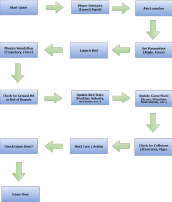
\includegraphics[width=0.5\linewidth]{Flowchartvnv.png}
    \caption{Flow chart diagram}
    \label{fig:enter-label}
\end{figure}

\end{document}
